%! Author = zhenxiang
%! Date = 23-3-26

\PassOptionsToPackage{quiet}{xeCJK}  % 抑制无意义的警告
% Preamble
\documentclass[11pt]{ctexart}


% Packages
\usepackage{amsmath}
% graphicx
\usepackage{graphicx}
% 页面设置
\usepackage{geometry}
\geometry{left=2.5cm, right=2.5cm, top=2.5cm, bottom=2.5cm}
% codes
\usepackage{listings}
\usepackage{xcolor}
\usepackage{color}
\definecolor{mygreen}{rgb}{0,0.6,0}
\definecolor{mygray}{rgb}{0.5,0.5,0.5}
\definecolor{mymauve}{rgb}{0.58,0,0.82}
\lstset{ %
	backgroundcolor=\color{white},   % choose the background color; you must add \usepackage{color} or \usepackage{xcolor}
	basicstyle=\ttfamily,            % the size of the fonts that are used for the code
	breakatwhitespace=false,         % sets if automatic breaks should only happen at whitespace
	breaklines=true,                 % sets automatic line breaking
	captionpos=b,                    % sets the caption-position to bottom
	commentstyle=\ttfamily\color{mygreen},    
	% comment style
	deletekeywords={},               % if you want to delete keywords from the given language
	escapeinside={},                 % if you want to add LaTeX within your code
	extendedchars=true,              % lets you use non-ASCII characters; for 8-bits encodings only, does not work with UTF-8
	frame=single,                    % adds a frame around the code
	keepspaces=true,                 % keeps spaces in text, useful for keeping indentation of code (possibly needs columns=flexible)
	keywordstyle=\color{blue},       % keyword style
	language=C++,                    % the language of the code
	morekeywords={},                 % if you want to add more keywords to the set
	numbers=left,                    % where to put the line-numbers; possible values are (none, left, right)
	numbersep=5pt,                   % how far the line-numbers are from the code
	numberstyle=\tiny\color{mygray}, % the style that is used for the line-numbers
	rulecolor=\color{black},         % if not set, the frame-color may be changed on line-breaks within not-black text (e.g. comments (green here))
	showspaces=false,                % show spaces everywhere adding particular underscores; it overrides 'showstringspaces'
	showstringspaces=false,          % underline spaces within strings only
	showtabs=false,                  % show tabs within strings adding particular underscores
	stepnumber=1,                    % the step between two line-numbers. If it's 1, each line will be numbered
	stringstyle=\color{mymauve},     % string literal style
	tabsize=2,                       % sets default tabsize to 2 spaces
	title=\lstname                   % show the filename of files included with \lstinputlisting; also try caption instead of title
}

% Document
\begin{document}

\section{lecture 3 Kernel-Based
	Data Parallel Execution Model}

\newpage
\section{Programming Massively Parallel Processors: Scalable parallel execution}

\subsection{CUDA THREAD ORGANIZATION}

In this chapter, we will study important concepts involved in the control of parallel execution. We will start by learning how thread index and block index can facilitate processing multidimensional arrays. Subsequently, we will explore the concept of flexible resource assignment and the concept of occupancy. We will then advance into thread scheduling, latency tolerance, and synchronization. A CUDA programmer who masters these concepts is
well-equipped to write and understand high-performance parallel applications.


\begin{lstlisting}
	// a 1D grid that consists of 32 blocks, each of which consists of 128 threads. The total number of threads in the grid is 128*32 = 4096.
	dim3 dimGrid(32, 1, 1);
	dim3 dimBlock(128, 1, 1);
	vecAddKernel<<<dimGrid, dimBlock>>>(…);
	//  the following statements accomplish the same as the statements above
	dim3 dog(32, 1, 1);
	dim3 cat(128, 1, 1);
	vecAddKernel<<<dog, cat>>>(…);
	// The grid and block dimensions can also be calculated from other variables.
	dim3 dimGrid(ceil(n/256.0), 1, 1);
	dim3 dimBlock(256, 1, 1);
	vecAddKernel<<<dimGrid, dimBlock>>>(…);
	
	
	//For convenience, CUDA C provides a special shortcut for launching a kernel with one-dimensional grids and blocks. Instead of dim3 variables, arithmetic expressions can be used to specify the configuration of 1D grids and blocks. 
	vecAddKernel<<<ceil(n/256.0), 256>>>(…);
\end{lstlisting}

Unlike the dim3 variables in  the host code, the name of these variables within the kernel functions are part of the CUDA C specification and cannot be changed --i.e., gridDim and blockDim in a kernel always reflect the dimensions of the grid and the blocks.

In CUDA C, the allowed values of gridDim.x, gridDim.y and  gridDim.z range from 1 to 65536. All threads in a block share the same blockid.x, blockidx.y, blockidx.z values.

Among blocks, the blockIdx.x value ranges from 0 to gridDim.x-1 , the blockIdx.y value from 0 to gridDim.y-1 , and the blockIdx.z
value from 0 to gridDim.z-1 .

The total size of a block is limited to 1024 threads, with flexibility in distributing
these elements into the three dimensions as long as the total number of threads does
not exceed 1024. For instance, blockDim(512, 1, 1) , blockDim(8, 16, 4), and
blockDim(32, 16, 2) are allowable blockDim values, but blockDim(32, 32, 2) is
not allowable because the total number of threads would exceed 1024.

The grid can have higher dimensionality than its blocks and vice versa. For
instance, code shows a small toy grid example of gridDim(2, 2, 1) with blockDim(4, 2, 2) . The grid can be generated with the following host code: 

\begin{lstlisting}
	dim3 dimGrid(2, 2, 1);
	dim3 dimBlock(4, 2, 2);
	KernelFunction<<<dimGrid, dimBlock>>>(…);
\end{lstlisting}

块 (1,0) 具有 blockIdx.y =1 和 blockIdx.x =0。这些标签的顺序是最高维度优先的。请注意,这种块标签符号是在设置配置参数的 C 语句中使用的符号顺序的反向顺序。在访问多维数据时,这种反向排序的块标记符号更有效。

% 图片置于当前位置
\begin{figure}[ht]
	\centering
	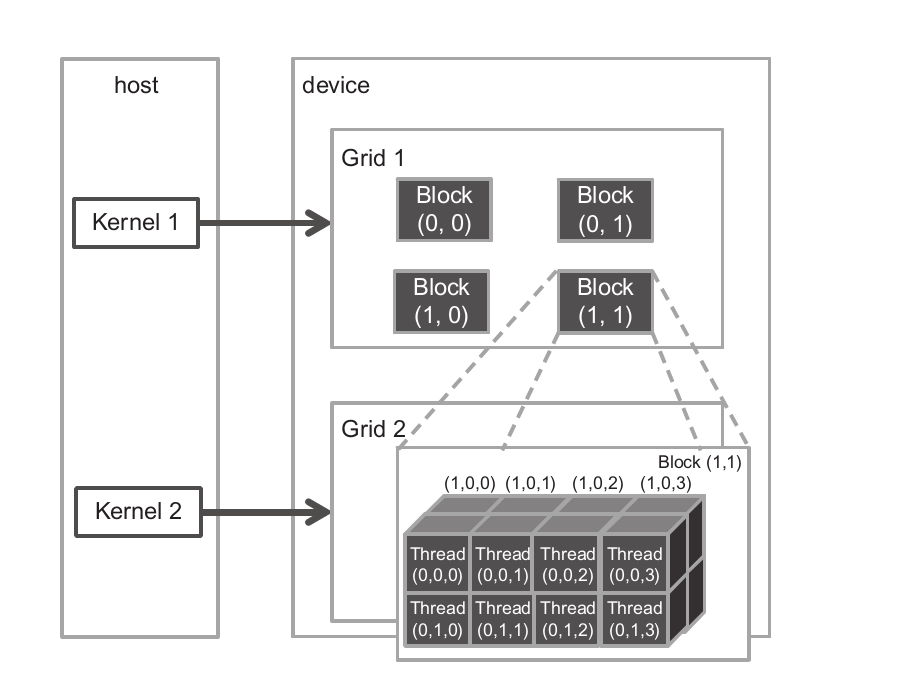
\includegraphics[width=1.0\textwidth]{photos/AmultidimensionalexampleofCUDAgridorganization.png}
	\caption{A multidimensional example of CUDA grid organization}
	\label{fig:1}
\end{figure}




每个 threadIdx 也由三个字段组成:x 坐标 threadId.x,y 坐标 threadIdx.y 和 z 坐标 threadIdx.z。图 3.1 展示了块内线程的组织方式。在此示例中,每个块组织成一个 4 × 2 × 2 的线程数组。所有网格中的块都具有相同的维度;因此,我们只需要显示其中一个。图 3.1 展开了块 (1,1),以显示其 16 个线程。例如,Thread(1,0,2) 具有 threadIdx.z=1、threadIdx.y=0 和 threadIdx.x=2。

Q:为什么这些标签的顺序是最高维度优先的?

A:在CUDA中,blockDim和gridDim参数是以最低维度优先的顺序定义的,这是因为在C语言中,多维数组的元素存储顺序也是以最低维度优先的顺序排列的。例如,对于一个二维数组A[i][j],内存中的数据排列顺序是按照j方向的索引连续存放的,即A[0][0]、A[0][1]、A[0][2]... A[1][0]、A[1][1]、A[1][2]... 以此类推。因此,在C语言中以最低维度优先的顺序定义数组和数据结构可以提高内存访问的效率。

然而,在CUDA中,blockIdx和threadIdx标签的顺序是以最高维度优先的顺序定义的,这是因为这种标签顺序更适合访问多维数组和其他多维数据结构。在CUDA中,每个线程都需要访问多维数组的一个元素,线程的坐标需要映射到数组的下标,因此使用最高维度优先的顺序可以简化这个映射过程,提高内存访问的效率。

使用最高维度优先的顺序可以简化映射过程,提高内存访问的效率,因为它与内存布局的方式是一致的。在计算机内存中,数据通常是按照一维数组的形式存储的,这意味着访问数组中的元素需要知道其索引在内存中的位置,索引的计算涉及到对内存地址的计算和寻址。按照最高维度优先的顺序标记块和线程可以让我们使用相同的索引计算方式来访问多维数据,这种方式可以减少计算量和寻址时间。

例如,假设我们要访问一个二维数组A[i][j],其中i表示行数,j表示列数。按照最高维度优先的顺序,我们可以将其表示为A[i * N + j],其中N表示数组中的列数。这样,我们可以使用相同的方式来访问一维数组和多维数组,并且不需要为每个数组定义一个不同的索引计算公式。

在CUDA程序中,我们通常需要在GPU内存中访问多维数组,按照最高维度优先的顺序标记块和线程可以简化对多维数组的索引计算,从而提高内存访问的效率。这种方法也使得并行程序员更容易处理多维数据,因为它使用了一种常见的编程惯例。

\subsection{MAPPING THREADS TO MULTIDIMENSIONAL DATA}

The choice of 1D, 2D, or 3D thread organizations is usually based on the nature of
the data. Pictures are 2D array of pixels. Using a 2D grid that consists of 2D blocks is
often convenient for processing the pixels in a picture.


Analogously, we should expect that the picture processing kernel function will have if statements to test whether the thread indexes threadIdx.x and threadIdx.y fall within the valid range of pixels.

\begin{lstlisting}
	dim3 dimGrid(ceil(m/16.0), ceil(n/16.0), 1);
	dim3 dimBlock(16, 16, 1);
	colorToGreyscaleConversion<<<dimGrid,dimBlock>>>(d_Pin,d_Pout,m,n);
\end{lstlisting}

\begin{equation}
	L = r * 0.21 + g * 0.72 + b * 0.07
\end{equation}

\begin{lstlisting}
	// we have 3 channels corresponding to RGB
	// The input image is encoded as unsigned characters [0, 255]
	__global__
	void colorToGreyscaleConversion(unsigned char * Pout, unsigned
	char * Pin, int width, int height) {,
		int Col = threadIdx.x + blockIdx.x * blockDim.x;
		int Row = threadIdx.y + blockIdx.y * blockDim.y;
		if (Col < width && Row < height) {
			// get 1D coordinate for the grayscale image
			int greyOffset = Row*width + Col;
			// one can think of the RGB image having
			// CHANNEL times columns than the grayscale image
			int rgbOffset = greyOffset*CHANNELS;
			unsigned char r = Pin[rgbOffset]; // red value for pixel
			unsigned char g = Pin[rgbOffset + 2]; // green value for pixel
			unsigned char b = Pin[rgbOffset + 3]; // blue value for pixel
			// perform the rescaling and store it
			// We multiply by floating point constants
			Pout[grayOffset] = 0.21f*r + 0.71f*g + 0.07f*b;
		}
	}
\end{lstlisting}

\subsection{IMAGE BLUR: A MORE COMPLEX KERNEL}

\begin{lstlisting}
	__global__
	void blurKernel(unsigned char * in, unsigned char * out, int w, int h){
			int Col  = blockIdx.x * blockDim.x + threadIdx.x;
			int Row = blockIdx.y * blockDim.y + threadIdx.y;
			
			if (Col < w && Row < h) {
				int pixVal = 0;
				int pixels = 0;	
				// Get the average of the surrounding BLUR_SIZE x BLUR_SIZE box
				for (int blurRow = - BLUR_SIZE; blurRow < BLUR_SIZE + 1; ++blurRow) {
						int curRow = Row + blurRow;
						int curCol = Col + blurCol;
						// Verify we have a valid image pixel
						if(curRow > -1 && curRow < h && curCol > -1 && curCol < w) {
								pixVal += in[curRow * w + curCol];
								pixels++; // Keep track of number of pixels in the avg	
					}		
			
			}
		}
		// Write our new pixel value out
		out[Row * w + Col] = (unsigned char)(pixVal /pixels); 

	}

}
\end{lstlisting}

\subsection{SYNCHRONIZATION AND TRANSPARENT SCALABILITY}

We have discussed thus far how to launch a kernel for execution by a grid of threads
and how to map threads to parts of the data structure. However, we have not yet presented any means to coordinate the execution of multiple threads. We will now study a basic coordination mechanism. CUDA allows threads in the same block to coordinate their activities by using a barrier synchronization function \_\_syncthreads() . Note that “\_\_” consists of two “\_” characters. When a thread calls \_\_syncthreads() , it will be held at the calling location until every thread in the block reaches the location. This process ensures that all threads in a block have completed a phase of their execution of the kernel before any of them can proceed to the next phase. Barrier synchronization is a simple and popular method for coordinating parallel activities.

In CUDA, a \_\_syncthreads() statement, if present, must be executed by all threads
in a block. When a \_\_syncthread() statement is placed in an if -statement, either all or none of the threads in a block execute the path that includes the \_\_syncthreads() . For an if-then-else statement, if each path has a \_\_syncthreads() statement, either all threads in a block execute the then -path or all of them execute the else -path. The two \_\_syncthreads() are different barrier synchronization points. If a thread in a block executes the then -path and another executes the else -path, they would be waiting at different barrier synchronization points. They would end up waiting for each other forever. It is the responsibility of the programmers to write their code so that these requirements are satisfied.

The ability to synchronize also imposes execution constraints on threads within a
block. These threads should execute in close temporal proximity with each other to
avoid excessively long waiting times. In fact, one needs to make sure that all threads
involved in the barrier synchronization have access to the necessary resources to eventually arrive at the barrier. Otherwise, a thread that never arrives at the barrier synchronization point can cause everyone else to wait forever. CUDA runtime systems satisfy this constraint by assigning execution resources to all threads in a block as a unit. A block can begin execution only when the runtime system has secured all resources needed for all threads in the block to complete execution. When a thread of a block is assigned to an execution resource, all other threads in the same block are also assigned to the same resource. This condition ensures the temporal proximity of all threads in a block and prevents excessive or indefinite waiting time during barrier synchronization.

This leads us to an important tradeoff in the design of CUDA barrier synchronization. By not allowing threads in different blocks to perform barrier synchronization
with each other, the CUDA runtime system can execute blocks in any order relative
to each other because none of them need to wait for each other. This flexibility ena-
bles scalable implementations as shown in Fig. 3.11, where time progresses from top
to bottom. In a low-cost system with only a few execution resources, one can execute
a small number of blocks simultaneously, portrayed as executing two blocks at a time
on the left hand side of Fig. 3.11. In a high-end implementation with more execution
resources, one can execute a large number of blocks simultaneously, shown as four
blocks at a time on the right hand side of Fig. 3.11.

% 图片置于当前位置
\begin{figure}[ht]
	\centering
	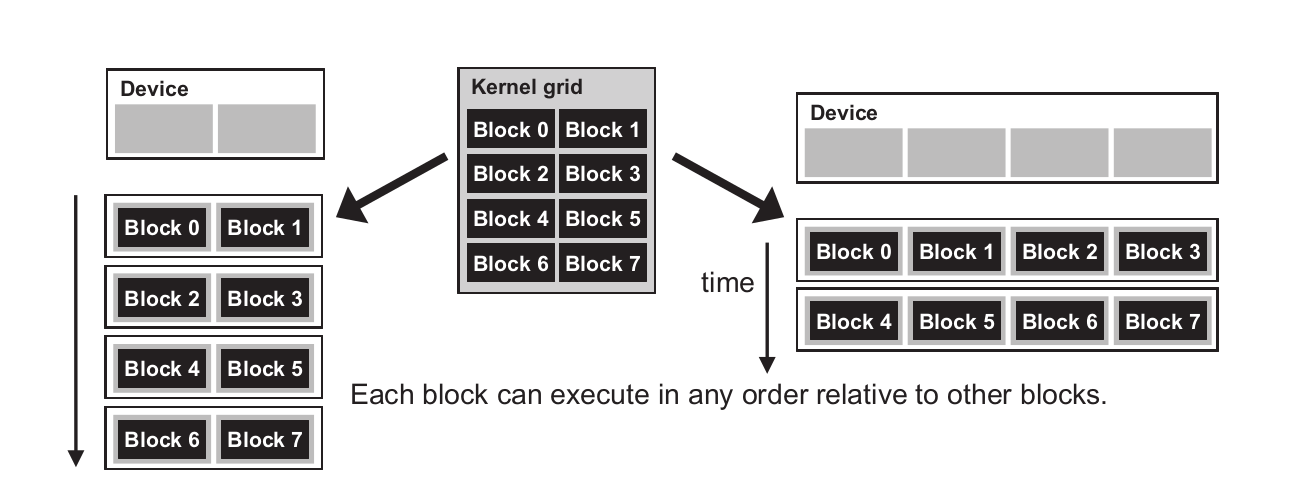
\includegraphics[width=1.0\textwidth]{photos/Lackofsynchronizationconstraints.png}
	\caption{Lackofsynchronizationconstraints.png}
	\label{fig:2}
\end{figure}


\subsection{RESOURCE ASSIGNMENT}

% 图片置于当前位置
\begin{figure}[ht]
	\centering
	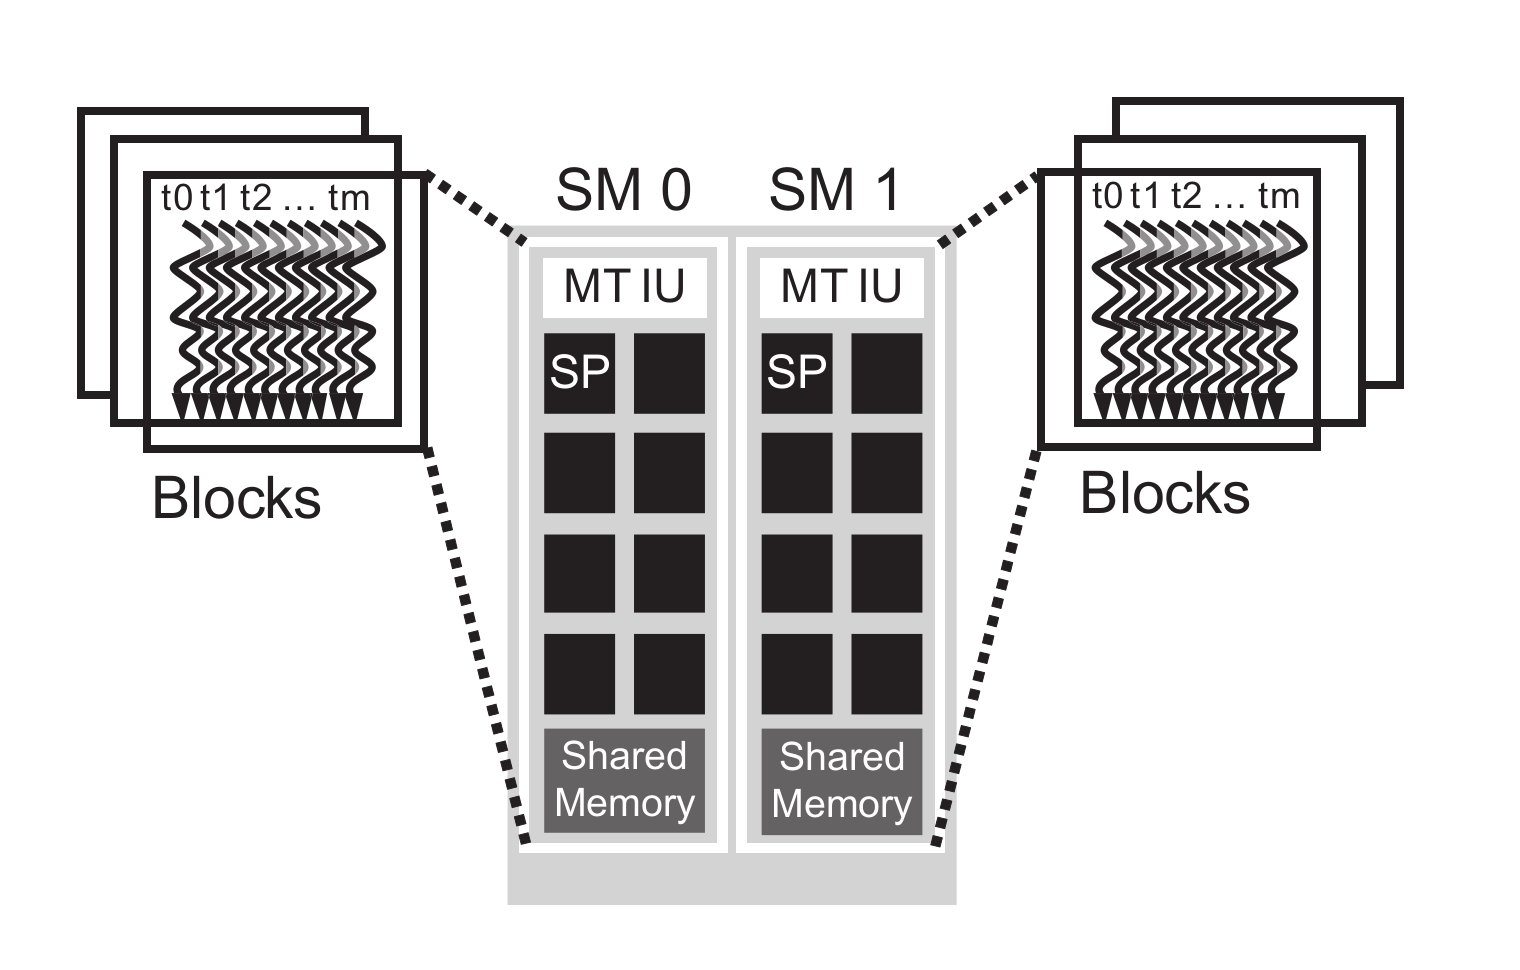
\includegraphics[width=1.0\textwidth]{photos/ThreadblockassignmenttoStreamingMultiprocessors.png}
	\caption{ThreadblockassignmenttoStreamingMultiprocessors.png}
	\label{fig:3}
\end{figure}



Once a kernel is launched, the CUDA runtime system generates the corresponding grid of threads. As discussed in the previous section, these threads are assigned to execution resources on a block-by-block basis. In the current generation of hardware, the execution resources are organized into Streaming Multiprocessors (SMs).
Fig. 3.12 illustrates that multiple thread blocks can be assigned to each SM. Each device sets a limit on the number of blocks that can be assigned to each SM. For instance, let us consider a CUDA device that may allow up to 8 blocks to be assigned to each SM. In situations where there is shortage of one or more types of resources needed for the simultaneous execution of 8 blocks, the CUDA runtime automatically reduces the number of blocks assigned to each SM until their combined resource usage falls below the limit. With limited numbers of SMs and limited numbers of blocks that can be assigned to each SM, the number of blocks that can be actively executing in a CUDA device is limited as well. Most grids contain many more blocks than this number. The runtime system maintains a list of blocks that need to execute and assigns new blocks to SMs as previously assigned blocks complete execution.
Fig. 3.12 shows an example in which three thread blocks are assigned to each SM.
One of the SM resource limitations is the number of threads that can be simultaneously tracked and scheduled. It takes hardware resources (built-in registers) for SMs to maintain the thread and block indexes and track their execution status. Therefore,
each generation of hardware sets a limit on the number of blocks and number of threads that can be assigned to an SM. For instance in the Fermi architecture, up to 8 blocks and 1536 threads can be assigned to each SM. This could be in the form of
6 blocks of 256 threads each, 3 blocks of 512 threads each, and so on. If the device only allows up to 8 blocks in an SM, it should be obvious that 12 blocks of 128 threads each is not a viable option. If a CUDA device has 30 SMs, and each SM can accommodate up to 1536 threads, the device can have up to 46,080 threads simultaneously residing in the CUDA device for execution.

Q: 
SM和线程的联系是什么?

A: 
在CUDA架构中,GPU的计算资源被组织成为一个个的Streaming Multiprocessors(SMs)。每个SM包含一组指令集、寄存器和其他硬件资源,可以同时处理多个线程块(thread blocks)中的线程(threads)。

线程是GPU并行计算的基本单元。一个线程块(thread block)是一组线程的集合,这些线程可以在同一个SM上并行执行。当一个CUDA内核启动时,系统会生成相应的线程网格。这些线程根据线程块的大小和分配方式被分配到SM上进行执行。

SM和线程之间的联系是,SM是GPU硬件上的执行单元,可以处理多个线程块中的线程。每个SM包含有限的资源,如寄存器和共享内存等,需要被分配给线程块中的线程使用。CUDA运行时系统会根据每个SM的资源限制,自动调整分配给每个SM的线程块数量,以确保所有线程可以被正确地分配和执行。因此,SM的数量和每个SM可以同时执行的线程数是GPU并行计算的两个重要的硬件限制。

\subsection{QUERYING DEVICE PROPERTIES}

Our discussions on assigning execution resources to blocks raise an important question. How do we find out the amount of resources available? When a CUDA application executes on a system, how can it determine the number of SMs in a device and the number of blocks and threads that can be assigned to each SM? Other resources have yet to be discussed that can be relevant to the execution of a CUDA application. In general, many modern applications are designed to execute on a wide variety of hardware systems. The application often needs to query the available resources and capabilities of the underlying hardware in order to take advantage of the more capable systems while compensating for the less capable systems.

In CUDA C, a built-in mechanism exists for a host code to query the properties of the devices available in the system. The CUDA runtime system (device driver) has an API function cudaGetDeviceCount that returns the number of available CUDA devices in the system. The host code can determine the number of available CUDA devices by using the following statements:

\begin{lstlisting}
	int dev_count;
	cudaGetDeviceCount(&dev_count);
\end{lstlisting}

A  modern PC system often has two  or more CUDA devices. The reason is that many PC systems come with one or more "intergrated" GPUs.These GPUs are the default graphics units and provide rudimentary capabilities and hardware resources to perform minimal graphics functionalities for modern Windows-based user interfaces. Most CUDA applications will not perform very well on these integrated devices. This weakness would be a reason for the host code to iterate through all the available devices, query their resources and capabilities, and choose the ones with adequate resources to execute the application satisfactorily.

The CUDA runtime numbers all available devices in the system from 0 to
dev\_count-1 . It provides an API function cudaGetDeviceProperties that returns the properties of the device whose number is given as an argument. We can use the following statements in the host code to iterate through the available devices and query their properties:

\begin{lstlisting}
	cudaDeviceProp dev_prop;
	for (int i = 0; i < dev_count; i++) {
		cudaGetDeviceProperties(&dev_prop, i);
		//decide if device has sufficient resources and capabilities
	}
\end{lstlisting}

The built-in type cudaDeviceProp is a C struct type with fields representing the properties of a CUDA device. The reader is referred to the CUDA C Programming Guide for all fields of the type. We will discuss a few of these fields that are particularly relevant to the assignment of execution resources to threads. We assume that the properties are returned in the dev\_prop variable whose fields are set by the cudaGetDeviceProperties function. If the reader chooses to name the variable differently,
the appropriate variable name will obviously need to be substituted in the following discussion.

As the name suggests, the field dev\_prop.maxThreadsPerBlock indicates the maximal number of threads allowed in a block in the queried device. Some devices allow up to 1024 threads in each block and other devices allow fewer. Future devices may even allow more than 1024 threads per block. Therefore, the available devices should be queried, and the ones that will allow a sufficient number of threads in each block should be determined. 

The number of SMs in the device is given in dev\_prop.multiProcessorCount . As we discussed earlier, some devices have only a small number of SMs (e.g., two) and some have a much larger number of SMs (e.g., 30). If the application requires a large number of SMs in order to achieve satisfactory performance, it should definitely
check this property of the prospective device. Furthermore, the clock frequency of the device is in dev\_prop.clockRate . The combination of the clock rate and the number of SMs provides a good indication of the hardware execution capacity of the device.

The host code can find the maximal number of threads allowed along each dimension of a block in fields dev\_prop.maxThreadsDim[0], dev\_prop.maxThreadsDim[1], and dev\_prop.maxThreadsDim[2] (for the x, y, and z dimensions).
Such information can be used for an automated tuning system to set the range of block dimensions when evaluating the best performing block dimensions for the  underlying hardware. Similarly, it can determine the maximal number of blocks allowed along each dimension of a grid in dev\_prop.maxGridSize[0] , dev\_prop.
maxGridSize[1] , and dev\_prop.maxGridSize[2] (for the x, y, and z dimensions). This information is typically used to determine whether a grid can have sufficient threads to handle the entire data set or whether some iteration is needed.

The cudaDeviceProp type has many more fields. We will discuss them as we
introduce the concepts and features that they are designed to reflect.

\subsection{THREAD SCHEDULING AND LATENCY TOLERANCE}

Thread scheduling is strictly an implementation concept. Thus, it must be discussed in the context of specific hardware implementations. In the majority of implementations to date, a block assigned to an SM is further divided into 32 thread units called warps. The size of warps is implementation-specific. Warps are not part of the CUDA specification; however, knowledge of warps can be helpful in understanding
and optimizing the performance of CUDA applications on particular generations of CUDA devices. The size of warps is a property of a CUDA device, which is in the warpSize field of the device query variable ( dev\_prop in this case).

The warp is the unit of thread scheduling in SMs. Fig. 3.13 shows the division
of blocks into warps in an implementation. Each warp consists of 32 threads of consecutive threadIdx values: thread 0 through 31 form the first warp, 32 through 63 the second warp, and so on. In this example, three blocks—Block 1, Block 2, and Block3—are assigned to an SM. Each of the three blocks is further divided into warps for scheduling purposes.

We can calculate the number of warps that reside in an SM for a given block size and a given number of blocks assigned to each SM. In Fig. 3.13, if each block has 256 threads, we can determine that each block has 256/32 or 8 warps. With three blocks in each SM, we have 8 × 3 = 24 warps in each SM.

An SM is designed to execute all threads in a warp following the Single
Instruction, Multiple Data (SIMD) model—i.e., at any instant in time, one instruction is fetched and executed for all threads in the warp. This situation is illustrated in Fig. 3.13 with a single instruction fetch/dispatch shared among execution units (SPs) in the SM. These threads will apply the same instruction to different portions of the data. Consequently, all threads in a warp will always have the same execution timing.

Fig. 3.13 also shows a number of hardware Streaming Processors (SPs) that actually execute instructions. In general, there are fewer SPs than the threads assigned to each SM; i.e., each SM has only enough hardware to execute instructions from a small subset of all threads assigned to the SM at any point in time. In early GPU designs, each SM can execute only one instruction for a single warp at any given instant. In recent designs, each SM can execute instructions for a small number of warps at any point in time. In either case, the hardware can execute instructions for a small subset of all warps in the SM. A legitimate question is why we need to have so many warps in an SM if it can only execute a small subset of them at any instant. The answer is that this is how CUDA processors efficiently execute long-latency operations, such as global memory accesses.

When an instruction to be executed by a warp needs to wait for the result of a previously initiated long-latency operation, the warp is not selected for execution.
Instead, another resident warp that is no longer waiting for results will be selected for execution. If more than one warp is ready for execution, a priority mechanism is used to select one for execution. This mechanism of filling the latency time of operations with work from other threads is often called “latency tolerance” or “latency hiding” (see “Latency Tolerance” sidebar).

Warp scheduling is also used for tolerating other types of operation latencies, such as pipelined floating-point arithmetic and branch instructions. Given a sufficient number of warps, the hardware will likely find a warp to execute at any point in time, thus making full use of the execution hardware in spite of these long-latency operations. The selection of ready warps for execution avoids introducing idle or wasted time into the execution timeline, which is referred to as zero-overhead thread
scheduling. With warp scheduling, the long waiting time of warp instructions is “hidden” by executing instructions from other warps. This ability to tolerate long-latency operations is the main reason GPUs do not dedicate nearly as much chip area to cache memories and branch prediction mechanisms as do CPUs. Thus, GPUs can dedicate more of its chip area to floating-point execution resources.

\textbf{LATENCY TOLERANCE} 延迟容忍性在日常生活中也是必需的。例如,在邮局中,每个试图寄送包裹的人理想情况下应该在前往服务柜台之前填写好所有必要的表格和标签。但是,有些人会等待服务台职员告诉他们应该填写哪个表格以及如何填写表格。

当服务柜台前排队的人很多时,服务员的生产率必须最大化。让一个人在所有人等待时在服务员面前填写表格不是一种高效的方法。服务员应该在那个人填写表格时帮助其他等待的顾客。这些其他顾客已经“准备好了”,不应该被需要更长时间填写表格的顾客阻塞。

因此,一个好的服务员会礼貌地要求第一个顾客在填写表格时离开服务柜台,这样他/她就可以为其他顾客提供服务。在大多数情况下,当该顾客完成表格并且服务员完成当前顾客的服务时,该顾客会立即被服务,而不是去排队的末尾。

我们可以将这些邮局顾客视为warp,将服务员视为硬件执行单元。需要填写表格的顾客对应于一个需要执行长延迟操作的warp。


现在我们来做一个简单的练习。假设一个CUDA设备每个SM最多可以容纳8个块和1024个线程,取决于先达到限制的那个。此外,它允许每个块最多有512个线程。对于图像模糊,我们应该使用8×8、16×16还是32×32的线程块?为了回答这个问题,我们可以分析每种选择的优缺点。如果我们使用8×8的块,每个块只有64个线程。我们将需要1024/64 = 12个块来充分占用一个SM。然而,每个SM只能允许最多8个块;因此,我们最终只能在每个SM中使用64×8 = 512个线程。这个有限的数量意味着SM执行资源可能会被低效利用,因为可用于在长延迟操作周围调度的warp较少。

16×16的块会产生256个线程,意味着每个SM可以容纳1024/256 = 4个块。这个数字在8块的限制范围内,并且是一个好的配置,因为它将允许我们在每个SM中拥有充分的线程容量和最大数量的warp来调度长延迟操作周围的线程。32×32的块会给出每个块1024个线程,超过了该设备每个块512个线程的限制。只有16×16的块允许每个SM分配最大数量的线程。

请注意,这只是一个过于简化的练习。正如我们将在第4章“内存和数据局部性”中解释的那样,在确定最适合的块维度时,还必须考虑\textbf{寄存器和共享内存}等其他资源的使用情况。此练习强调了块数限制和每个SM可分配的线程数限制之间的相互作用。

\subsection{SUMMARY}

The kernel execution configuration parameters define the dimensions of a grid and its blocks. Unique coordinates in blockIdx and threadIdx allow threads of a grid to identify themselves and their domains of data. It is the responsibility of the programmer to use these variables in kernel functions so that the threads can properly identify the portion of the data to process. This model of programming compels the programmer to organize threads and their data into hierarchical and multidimensional organizations.

Once a grid is launched, its blocks can be assigned to SMs in an arbitrary order, resulting in the transparent scalability of CUDA applications. The transparent scalability comes with a limitation: threads in different blocks cannot synchronize with
one another. To allow a kernel to maintain transparent scalability, the simple method
for threads in different blocks to synchronize with each other is to terminate the ker-
nel and start a new kernel for the activities after the synchronization point.

Threads are assigned to SMs for execution on a block-by-block basis. Each CUDA
device imposes a potentially different limitation on the amount of resources available
in each SM. Each CUDA device sets a limit on the number of blocks and the number
of threads each of its SMs can accommodate, whichever becomes a limitation first.
For each kernel, one or more of these resource limitations can become the limiting
factor for the number of threads that simultaneously reside in a CUDA device.

Once a block is assigned to an SM, it is further partitioned into warps. All threads
in a warp have identical execution timing. At any time, the SM executes instruc-
tions of only a small subset of its resident warps. This condition allows the other
warps to wait for long-latency operations without slowing down the overall execu-
tion throughput of the massive number of execution units.

Q: 详说不同块中的线程进行同步的简单方法

A:在CUDA中,不同块中的线程不能直接进行同步,因为它们分别被分配到不同的SM中运行。然而,有一种简单的方法,可以让不同块中的线程进行同步,即在同步点处终止当前的kernel函数并启动一个新的kernel函数。

具体地说,当需要进行同步时,可以在kernel函数的某个位置使用CUDA提供的同步函数(如\_\_syncthreads())来进行同步。在这个同步函数被调用的位置,所有线程都会停止执行,等待其他块中的线程完成它们的任务。一旦所有线程都到达同步点,kernel函数会终止,并启动一个新的kernel函数,来执行同步点之后的任务。

需要注意的是,这种方法虽然简单,但是会带来一定的开销,因为在进行同步时需要启动一个新的kernel函数。此外,由于每个kernel函数的启动都需要一定的时间,所以频繁的kernel函数启动也会降低程序的性能。因此,在实际编程中,需要根据具体的应用场景,选择合适的同步策略,以达到最佳的性能和效率。


\end{document}